% =====================================================================
%  Capítulo 3. Regresión lineal en finanzas: modelo de mercado y CAPM
% =====================================================================
\chapter{Regresión lineal en finanzas: el modelo de mercado y el CAPM}\label{cap:capm}

\section*{Objetivos de aprendizaje}
Al terminar este capítulo, el lector podrá:
\begin{enumerate}[label=\arabic*.,leftmargin=*]
  \item Estimar por mínimos cuadrados ordinarios (MCO) el modelo de mercado y derivar las fórmulas de los
        estimadores, sus varianzas y su optimalidad (teorema de Gauss-Markov).
  \item Descomponer el riesgo total de un activo en riesgo sistemático e idiosincrático, e interpretar el
        $R^2$ en esos términos.
  \item Demostrar que la relación beta-rendimiento esperado se cumple para cualquier portafolio eficiente
        en media-varianza, y entender el CAPM como la afirmación de que el portafolio de mercado lo es.
  \item Contrastar el CAPM en series de tiempo (alfas) y en corte transversal (recta del mercado de
        valores), y reconocer sus limitaciones (inestabilidad de las betas, crítica de Roll).
\end{enumerate}

\section*{Motivación}
Si un fondo de pensiones peruano gana 12\,\% en un año en que la Bolsa sube 15\,\%, ¿lo hizo bien o mal?
La respuesta depende del riesgo que asumió. El \emph{modelo de mercado} mide ese riesgo con un solo
número, la \emph{beta}: cuánto se mueve el activo cuando se mueve el mercado. El \emph{CAPM} (modelo de
valoración de activos de capital, de Sharpe, Lintner y Mossin) va más lejos y afirma que la beta es lo
único que el mercado premia: dos activos con la misma beta deberían tener el mismo rendimiento esperado,
por distintos que sean en todo lo demás. Es el modelo más usado en la práctica para calcular el costo de
capital de una empresa, para evaluar gestores de fondos y como referencia en la regulación tarifaria
(por ejemplo, para fijar la rentabilidad permitida de empresas de servicios públicos).

Este capítulo desarrolla la herramienta econométrica (la regresión lineal por MCO), demuestra el
resultado teórico central (la relación beta-rendimiento) y somete el modelo a prueba con casi 70 años de
datos reales.

\paragraph{Datos del capítulo.} Usamos la base de datos de Kenneth R. French (Dartmouth College), la
referencia estándar en finanzas empíricas: rendimientos mensuales de enero de 1949 a marzo de 2017 (819
meses) del mercado accionario de EE.\,UU., de la tasa libre de riesgo (letra del Tesoro a un mes) y de
12 portafolios por industria. Usamos la copia incluida en el paquete de Python \texttt{linearmodels}, que
termina en marzo de 2017; los resultados de este capítulo valen para ese período. Las aplicaciones a
acciones peruanas (Credicorp, Southern Copper y Buenaventura frente al índice de la BVL) se plantean como
ejercicios propuestos con los datos del Capítulo~\ref{cap:rendimientos}.

% ---------------------------------------------------------------------
\section{El modelo de mercado}
% ---------------------------------------------------------------------

Sea $R_{it}$ el rendimiento simple del activo $i$ en el mes $t$, $R_{mt}$ el del portafolio de mercado y
$R_{ft}$ la tasa libre de riesgo del mes, conocida al inicio. Trabajamos con \emph{excesos de rendimiento}
(Definición~\ref{def:exceso}): $Z_{it}=R_{it}-R_{ft}$ y $Z_{mt}=R_{mt}-R_{ft}$.

\begin{definicion}[Modelo de mercado]
El modelo de mercado postula que
\[
  Z_{it}=\alpha_i+\beta_i Z_{mt}+\varepsilon_{it},\qquad \E[\varepsilon_{it}]=0,\qquad
  \Cov(Z_{mt},\varepsilon_{it})=0 .
\]
La pendiente $\beta_i$ es la \emph{beta} del activo, la ordenada $\alpha_i$ es su \emph{alfa de Jensen}
y $\varepsilon_{it}$ es el componente \emph{idiosincrático}: la parte del rendimiento que no se explica por
el mercado.
\end{definicion}

\begin{proposicion}[Beta poblacional]\label{prop:betapob}
Bajo los supuestos del modelo de mercado,
\[
  \beta_i=\frac{\Cov(Z_{it},Z_{mt})}{\Var(Z_{mt})},\qquad \alpha_i=\E[Z_{it}]-\beta_i\,\E[Z_{mt}] .
\]
\end{proposicion}

\begin{proof}
Tomando esperanzas en el modelo, con $\E[\varepsilon_{it}]=0$:
\begin{align*}
  \E[Z_{it}] &= \alpha_i+\beta_i\,\E[Z_{mt}]+\E[\varepsilon_{it}]\\
             &= \alpha_i+\beta_i\,\E[Z_{mt}],\\
  \alpha_i   &= \E[Z_{it}]-\beta_i\,\E[Z_{mt}].
\end{align*}
Tomando la covarianza de ambos lados con $Z_{mt}$, y usando que la covarianza con una constante es cero y
que $\Cov(Z_{mt},\varepsilon_{it})=0$:
\begin{align*}
  \Cov(Z_{it},Z_{mt}) &= \Cov(\alpha_i+\beta_iZ_{mt}+\varepsilon_{it},\ Z_{mt})\\
                      &= 0+\beta_i\Var(Z_{mt})+\Cov(\varepsilon_{it},Z_{mt})\\
                      &= \beta_i\Var(Z_{mt}),\\
  \beta_i             &= \frac{\Cov(Z_{it},Z_{mt})}{\Var(Z_{mt})}. && \qedhere
\end{align*}
\end{proof}

\begin{proposicion}[Descomposición del riesgo]\label{prop:descriesgo}
La varianza del exceso de rendimiento se descompone en
\[
  \underbrace{\Var(Z_{it})}_{\text{riesgo total}}=\underbrace{\beta_i^2\Var(Z_{mt})}_{\text{riesgo sistemático}}
  +\underbrace{\Var(\varepsilon_{it})}_{\text{riesgo idiosincrático}},
\]
y la proporción de riesgo sistemático es $R^2_i=\beta_i^2\Var(Z_{mt})/\Var(Z_{it})=\rho^2(Z_{it},Z_{mt})$,
el cuadrado de la correlación entre el activo y el mercado.
\end{proposicion}

\begin{proof}
Como $Z_{mt}$ y $\varepsilon_{it}$ no están correlacionados:
\begin{align*}
  \Var(Z_{it}) &= \Var(\alpha_i+\beta_iZ_{mt}+\varepsilon_{it})\\
               &= \beta_i^2\Var(Z_{mt})+\Var(\varepsilon_{it})+2\beta_i\Cov(Z_{mt},\varepsilon_{it})\\
               &= \beta_i^2\Var(Z_{mt})+\Var(\varepsilon_{it}).
\end{align*}
Para la segunda afirmación, sustituimos la beta de la Proposición~\ref{prop:betapob}:
\begin{align*}
  R_i^2 &= \frac{\beta_i^2\Var(Z_{mt})}{\Var(Z_{it})}\\
        &= \frac{\Cov(Z_{it},Z_{mt})^2}{\Var(Z_{mt})^2}\cdot\frac{\Var(Z_{mt})}{\Var(Z_{it})}\\
        &= \frac{\Cov(Z_{it},Z_{mt})^2}{\Var(Z_{mt})\,\Var(Z_{it})}\\
        &= \rho^2(Z_{it},Z_{mt}). && \qedhere
\end{align*}
\end{proof}

La distinción es económicamente crucial. El riesgo idiosincrático se puede eliminar diversificando: en un
portafolio de muchos activos, los $\varepsilon_{it}$ independientes se promedian y su varianza tiende a cero.
El riesgo sistemático no se diversifica, porque todos los activos dependen del mismo $Z_{mt}$. Por eso,
según el CAPM, solo el riesgo sistemático debe ser compensado con un rendimiento esperado mayor. La
Figura~\ref{fig:riesgo} muestra dos activos con la misma beta y riesgos idiosincráticos muy distintos: un
inversionista diversificado debería exigirles el mismo rendimiento.

\begin{figure}[ht]
\centering
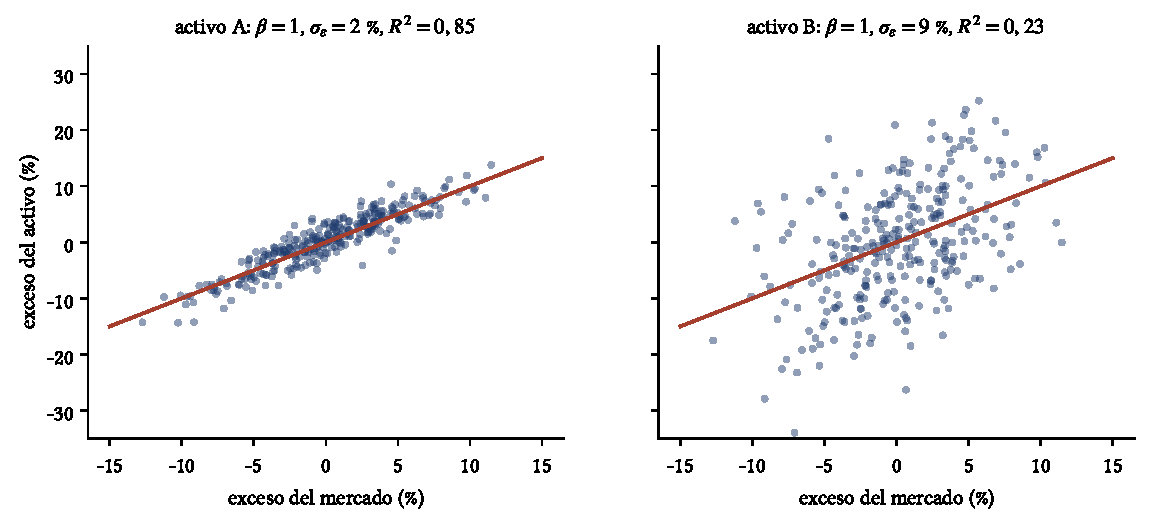
\includegraphics[width=\linewidth]{graficos/cap03_fig_riesgo.pdf}
\caption{Dos activos simulados con la misma beta ($\beta=1$, recta roja) y distinto riesgo idiosincrático.
En A los puntos se pegan a la recta: casi todo su riesgo es sistemático ($R^2$ alto). En B la nube es
mucho más ancha: la mayor parte de su riesgo es idiosincrático y desaparece en un portafolio diversificado.}
\label{fig:riesgo}
\end{figure}

% ---------------------------------------------------------------------
\section{Estimación por mínimos cuadrados ordinarios}
% ---------------------------------------------------------------------

Con una muestra $(x_t,y_t)$, $t=1,\dots,T$, donde $y_t=Z_{it}$ y $x_t=Z_{mt}$, escribimos
$\bar x,\bar y$ para las medias muestrales,
$S_{xx}=\sum_t(x_t-\bar x)^2$ y $S_{xy}=\sum_t(x_t-\bar x)(y_t-\bar y)$.

\begin{proposicion}[Estimadores MCO]\label{prop:mco}
Los valores $(\hat\alpha,\hat\beta)$ que minimizan la suma de residuos al cuadrado
$\mathrm{SRC}(a,b)=\sum_t(y_t-a-bx_t)^2$ son
\[
  \hat\beta=\frac{S_{xy}}{S_{xx}},\qquad \hat\alpha=\bar y-\hat\beta\,\bar x .
\]
\end{proposicion}

\begin{proof}
$\mathrm{SRC}$ es una función cuadrática convexa de $(a,b)$, así que su mínimo está donde se anulan las
derivadas parciales:
\begin{align}
  \frac{\partial\,\mathrm{SRC}}{\partial a} &= -2\sum_t(y_t-a-bx_t)=0, \tag{i}\\
  \frac{\partial\,\mathrm{SRC}}{\partial b} &= -2\sum_tx_t(y_t-a-bx_t)=0. \tag{ii}
\end{align}
De (i):
\begin{align*}
  \sum_ty_t-Ta-b\sum_tx_t &= 0\\
  T\bar y-Ta-bT\bar x &= 0\\
  a &= \bar y-b\,\bar x .
\end{align*}
Sustituyendo $a$ en (ii):
\begin{align*}
  \sum_tx_t\bigl(y_t-\bar y+b\bar x-bx_t\bigr) &= 0\\
  \sum_tx_t(y_t-\bar y)-b\sum_tx_t(x_t-\bar x) &= 0\\
  \sum_t(x_t-\bar x)(y_t-\bar y)-b\sum_t(x_t-\bar x)^2 &= 0\\
  S_{xy}-b\,S_{xx} &= 0\\
  b &= \frac{S_{xy}}{S_{xx}} .
\end{align*}
En la tercera línea restamos $\bar x$ dentro de cada suma, lo que no cambia nada porque
$\sum_t\bar x(y_t-\bar y)=0$ y $\sum_t\bar x(x_t-\bar x)=0$.
\end{proof}

La fórmula es la contraparte muestral de la Proposición~\ref{prop:betapob}: covarianza muestral entre
varianza muestral. La Figura~\ref{fig:mco} muestra qué significa ``minimizar la suma de residuos al
cuadrado'': de todas las rectas posibles, MCO elige la que hace más pequeña la suma de los cuadrados de
las distancias \emph{verticales} entre los puntos y la recta.

\begin{figure}[ht]
\centering
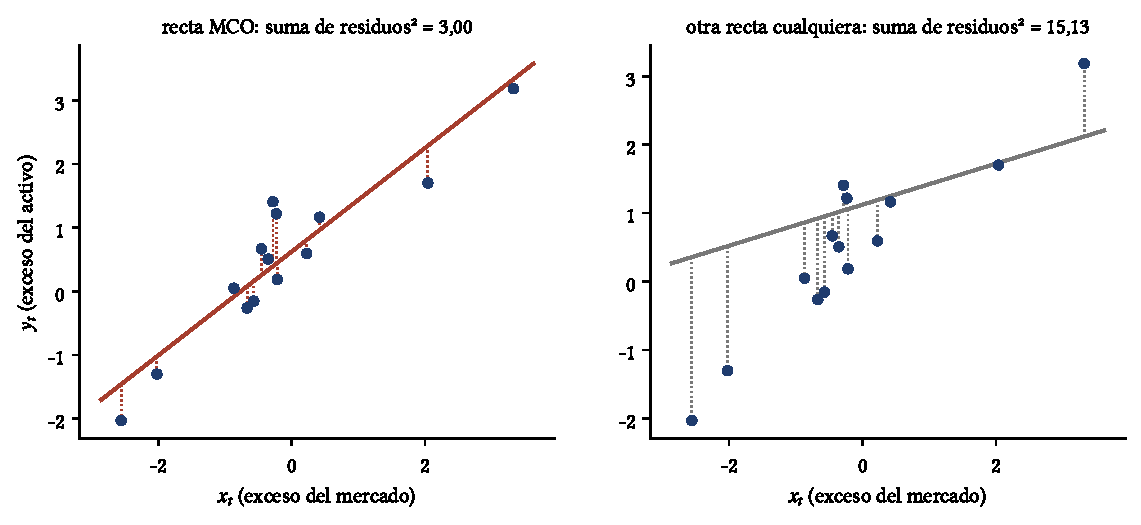
\includegraphics[width=\linewidth]{graficos/cap03_fig_mco.pdf}
\caption{Los residuos son las distancias verticales (líneas punteadas) entre cada observación y la recta.
La recta MCO (izquierda) tiene una suma de residuos al cuadrado de 3,00; cualquier otra recta, como la
de la derecha, tiene una suma mayor (aquí, 15,13). Datos simulados.}
\label{fig:mco}
\end{figure}

\begin{teorema}[Insesgamiento y varianza]\label{teo:varmco}
Suponga que $y_t=\alpha+\beta x_t+\varepsilon_t$ con $\E[\varepsilon_t\mid x_1,\dots,x_T]=0$,
$\Var(\varepsilon_t\mid x)=\sigma^2$ y $\Cov(\varepsilon_t,\varepsilon_s\mid x)=0$ para $t\ne s$. Entonces,
condicional en $x=(x_1,\dots,x_T)$,
\[
  \E[\hat\beta\mid x]=\beta,\qquad \Var(\hat\beta\mid x)=\frac{\sigma^2}{S_{xx}},\qquad
  \Var(\hat\alpha\mid x)=\sigma^2\Bigl(\frac1T+\frac{\bar x^2}{S_{xx}}\Bigr).
\]
\end{teorema}

\begin{proof}
Definimos los pesos $c_t=(x_t-\bar x)/S_{xx}$. Cumplen tres propiedades:
\begin{align*}
  \sum_tc_t    &= \frac{\sum_t(x_t-\bar x)}{S_{xx}} = 0,\\
  \sum_tc_tx_t &= \frac{\sum_t(x_t-\bar x)x_t}{S_{xx}} = \frac{\sum_t(x_t-\bar x)^2}{S_{xx}} = 1,\\
  \sum_tc_t^2  &= \frac{\sum_t(x_t-\bar x)^2}{S_{xx}^2} = \frac{1}{S_{xx}} .
\end{align*}
Como $\sum_t(x_t-\bar x)=0$, se cumple $S_{xy}=\sum_t(x_t-\bar x)y_t$, y entonces
\begin{align*}
  \hat\beta &= \sum_tc_ty_t\\
            &= \sum_tc_t\,(\alpha+\beta x_t+\varepsilon_t)\\
            &= \alpha\sum_tc_t+\beta\sum_tc_tx_t+\sum_tc_t\varepsilon_t\\
            &= \alpha\cdot0+\beta\cdot1+\sum_tc_t\varepsilon_t\\
            &= \beta+\sum_tc_t\varepsilon_t .
\end{align*}
Como los $c_t$ dependen solo de $x$:
\begin{align*}
  \E[\hat\beta\mid x] &= \beta+\sum_tc_t\,\E[\varepsilon_t\mid x]\\
                      &= \beta,\\
  \Var(\hat\beta\mid x) &= \sum_tc_t^2\,\Var(\varepsilon_t\mid x)\\
                        &= \sigma^2\sum_tc_t^2\\
                        &= \frac{\sigma^2}{S_{xx}} .
\end{align*}
Para $\hat\alpha$, con $\bar\varepsilon=\frac1T\sum_t\varepsilon_t$:
\begin{align*}
  \hat\alpha &= \bar y-\hat\beta\,\bar x\\
             &= (\alpha+\beta\bar x+\bar\varepsilon)-\hat\beta\,\bar x\\
             &= \alpha+\bar\varepsilon-(\hat\beta-\beta)\,\bar x .
\end{align*}
Los dos términos aleatorios no están correlacionados:
\begin{align*}
  \Cov(\bar\varepsilon,\hat\beta\mid x) &= \Cov\Bigl(\frac1T\sum_t\varepsilon_t,\ \sum_tc_t\varepsilon_t\Bigm|x\Bigr)\\
                                        &= \frac{\sigma^2}{T}\sum_tc_t\\
                                        &= 0 .
\end{align*}
Por tanto,
\begin{align*}
  \Var(\hat\alpha\mid x) &= \Var(\bar\varepsilon\mid x)+\bar x^2\,\Var(\hat\beta\mid x)\\
                         &= \frac{\sigma^2}{T}+\frac{\bar x^2\sigma^2}{S_{xx}}\\
                         &= \sigma^2\Bigl(\frac1T+\frac{\bar x^2}{S_{xx}}\Bigr). && \qedhere
\end{align*}
\end{proof}

\begin{teorema}[Gauss-Markov]\label{teo:gm}
Bajo los supuestos del Teorema~\ref{teo:varmco}, $\hat\beta$ tiene la menor varianza entre todos los
estimadores de $\beta$ que son lineales en $y$ e insesgados.
\end{teorema}

\begin{proof}
Sea $\tilde\beta=\sum_tk_ty_t$, con pesos $k_t$ que dependen solo de $x$. Su esperanza es
\begin{align*}
  \E[\tilde\beta\mid x] &= \sum_tk_t\,\E[y_t\mid x]\\
                        &= \sum_tk_t\,(\alpha+\beta x_t)\\
                        &= \alpha\sum_tk_t+\beta\sum_tk_tx_t .
\end{align*}
Para que sea igual a $\beta$ con cualquier $(\alpha,\beta)$ se necesita $\sum_tk_t=0$ y $\sum_tk_tx_t=1$. Su
varianza es $\Var(\tilde\beta\mid x)=\sigma^2\sum_tk_t^2$. Escribimos $k_t=c_t+d_t$, con los $c_t$ de MCO.
Como $k_t$ y $c_t$ cumplen las mismas dos restricciones:
\begin{align*}
  \sum_td_t    &= \sum_tk_t-\sum_tc_t = 0-0 = 0,\\
  \sum_td_tx_t &= \sum_tk_tx_t-\sum_tc_tx_t = 1-1 = 0,
\end{align*}
y entonces
\begin{align*}
  \sum_tc_td_t &= \frac{1}{S_{xx}}\sum_t(x_t-\bar x)\,d_t\\
               &= \frac{1}{S_{xx}}\Bigl(\sum_tx_td_t-\bar x\sum_td_t\Bigr)\\
               &= \frac{1}{S_{xx}}\,(0-0)\\
               &= 0 .
\end{align*}
Por tanto,
\begin{align*}
  \sum_tk_t^2 &= \sum_t(c_t+d_t)^2\\
              &= \sum_tc_t^2+2\sum_tc_td_t+\sum_td_t^2\\
              &= \frac{1}{S_{xx}}+0+\sum_td_t^2\\
              &\ge \frac{1}{S_{xx}},
\end{align*}
con igualdad solo si todos los $d_t$ son cero, es decir, si $\tilde\beta=\hat\beta$.
\end{proof}

\begin{proposicion}[Inferencia]\label{prop:inferencia}
Con $\hat\varepsilon_t=y_t-\hat\alpha-\hat\beta x_t$ y $s^2=\frac{1}{T-2}\sum_t\hat\varepsilon_t^2$, los
errores estándar son $\operatorname{ee}(\hat\beta)=\sqrt{s^2/S_{xx}}$ y
$\operatorname{ee}(\hat\alpha)=\sqrt{s^2(1/T+\bar x^2/S_{xx})}$. Si además los errores son normales,
$(\hat\beta-\beta)/\operatorname{ee}(\hat\beta)\sim t_{T-2}$ y lo mismo para $\hat\alpha$; sin
normalidad, el resultado vale asintóticamente con la normal estándar.
\end{proposicion}

Omitimos la demostración, que es estándar (véase Wooldridge, 2020, cap.~4). Lo importante para este
capítulo es su alcance: los errores estándar de la Proposición~\ref{prop:inferencia} suponen
homocedasticidad y ausencia de autocorrelación. El Capítulo~\ref{cap:hechos} mostró que los rendimientos
financieros tienen volatilidad cambiante; en el Capítulo~4 repetiremos las pruebas de este capítulo con
errores estándar robustos.

% ---------------------------------------------------------------------
\section{El CAPM}
% ---------------------------------------------------------------------

\subsection{La relación beta-rendimiento para un portafolio eficiente}

Considere $N$ activos riesgosos con vector de excesos de rendimiento esperados $\bm\mu$ (de dimensión
$N\times1$) y matriz de covarianzas $\bm\Sigma$, invertible, además de un activo libre de riesgo. Un
portafolio con pesos $\bm w$ en los activos riesgosos (y $1-\bm w'\bm1$ en el libre de riesgo) tiene
exceso esperado $\bm w'\bm\mu$ y varianza $\bm w'\bm\Sigma\bm w$. Un portafolio es \emph{eficiente} si
tiene la mínima varianza entre todos los que tienen su mismo exceso esperado.

\begin{teorema}[Relación beta-rendimiento]\label{teo:betarend}
Sea $q$ un portafolio eficiente con exceso esperado $\mu_q>0$. Entonces, para todo activo $i$,
\[
  \mu_i=\beta_{iq}\,\mu_q,\qquad \beta_{iq}=\frac{\Cov(Z_i,Z_q)}{\Var(Z_q)} .
\]
\end{teorema}

\begin{proof}
El portafolio eficiente resuelve $\min_{\bm w}\ \tfrac12\bm w'\bm\Sigma\bm w$ sujeto a
$\bm w'\bm\mu=\mu_q$. El lagrangiano y su condición de primer orden son
\begin{align*}
  \mathcal L &= \tfrac12\,\bm w'\bm\Sigma\bm w-\lambda\,(\bm w'\bm\mu-\mu_q),\\
  \frac{\partial\mathcal L}{\partial\bm w} &= \bm\Sigma\bm w-\lambda\bm\mu=\bm0,\\
  \bm\Sigma\bm w_q &= \lambda\,\bm\mu .
\end{align*}
Como $Z_q=\bm w_q'\bm Z$, la componente $i$ de $\bm\Sigma\bm w_q$ es la covarianza entre el activo $i$ y
el portafolio $q$:
\begin{equation}
  \Cov(Z_i,Z_q)=(\bm\Sigma\bm w_q)_i=\lambda\,\mu_i . \tag{a}
\end{equation}
Premultiplicando la condición de primer orden por $\bm w_q'$:
\begin{align*}
  \bm w_q'\bm\Sigma\bm w_q &= \lambda\,\bm w_q'\bm\mu\\
  \Var(Z_q)                &= \lambda\,\mu_q\\
  \lambda                  &= \frac{\Var(Z_q)}{\mu_q} .
\end{align*}
Sustituyendo $\lambda$ en (a):
\begin{align*}
  \mu_i &= \frac{\Cov(Z_i,Z_q)}{\lambda}\\
        &= \frac{\Cov(Z_i,Z_q)}{\Var(Z_q)}\,\mu_q\\
        &= \beta_{iq}\,\mu_q . && \qedhere
\end{align*}
\end{proof}

\begin{corolario}[Portafolio tangente]\label{cor:tangente}
De la demostración, todo portafolio eficiente tiene pesos proporcionales a $\bm\Sigma^{-1}\bm\mu$. El
portafolio eficiente formado solo por activos riesgosos (pesos que suman uno) es el \emph{portafolio
tangente}, $\bm w_q=\bm\Sigma^{-1}\bm\mu/(\bm1'\bm\Sigma^{-1}\bm\mu)$, y su razón de Sharpe es la máxima posible:
$\mu_q/\sigma_q=\sqrt{\bm\mu'\bm\Sigma^{-1}\bm\mu}$.
\end{corolario}

El Teorema~\ref{teo:betarend} es un resultado \emph{matemático}: vale para cualquier conjunto de activos y
cualquier portafolio eficiente, sin supuestos sobre el comportamiento de los inversionistas. El
\emph{contenido económico} del CAPM es la afirmación adicional de que, en equilibrio, si todos los
inversionistas optimizan en media-varianza con las mismas expectativas, el portafolio de mercado es el
portafolio tangente. Entonces $\mu_i=\beta_{im}\mu_m$ para todo activo: la \emph{recta del mercado de
valores} (SML, por sus siglas en inglés). La Figura~\ref{fig:capm} muestra la geometría: a la izquierda,
el portafolio tangente es el punto donde la recta que sale del activo libre de riesgo toca la frontera
eficiente; a la derecha, la SML y lo que significa una alfa distinta de cero.

\begin{figure}[ht]
\centering
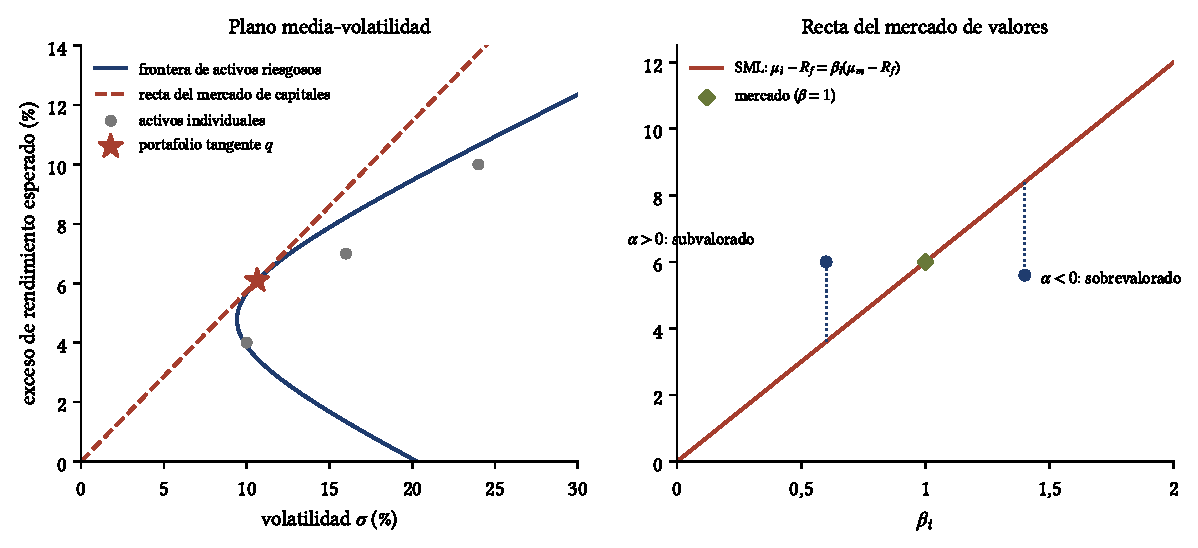
\includegraphics[width=\linewidth]{graficos/cap03_fig_capm.pdf}
\caption{Izquierda: la frontera de mínima varianza de tres activos riesgosos (parámetros ilustrativos) es
una hipérbola; la recta que parte del activo libre de riesgo y es tangente a ella (recta del mercado de
capitales) da la mejor relación entre riesgo y rendimiento, y toca la frontera en el portafolio tangente.
Derecha: la SML. Un activo por encima de ella ($\alpha>0$) rinde más de lo que su beta justifica; uno por
debajo ($\alpha<0$), menos.}
\label{fig:capm}
\end{figure}

\subsection{Cómo se contrasta}

En el modelo de mercado, tomando esperanzas, $\E[Z_{it}]=\alpha_i+\beta_i\E[Z_{mt}]$. Comparando con la
SML, \emph{el CAPM equivale a $\alpha_i=0$ para todo activo}. Esto da dos maneras de contrastarlo:
\begin{enumerate}[label=(\roman*),leftmargin=*]
  \item \textbf{En series de tiempo:} estimar el modelo de mercado para cada activo y probar
        $H_0:\alpha_i=0$ con el estadístico $t$. La prueba conjunta para todos los activos (Gibbons, Ross
        y Shanken, 1989) se estudia en el Capítulo~14.
  \item \textbf{En corte transversal:} estimar primero las betas y luego regresar los excesos de
        rendimiento promedio sobre ellas, $\bar Z_i=\gamma_0+\gamma_1\hat\beta_i+u_i$. El CAPM predice
        $\gamma_0=0$ y $\gamma_1=\bar Z_m$ (la prima de mercado).
\end{enumerate}

\begin{observacion}[La crítica de Roll]
Roll (1977) señaló que, por el Teorema~\ref{teo:betarend}, contrastar el CAPM es lo mismo que contrastar si
el portafolio usado como ``mercado'' es eficiente. Como el verdadero portafolio de mercado incluye todos los
activos de la economía (acciones, bonos, inmuebles, capital humano), y en la práctica se usa un índice
bursátil, un rechazo puede deberse a que el índice no es el mercado verdadero. Ilustraremos este punto en
el Ejercicio~\ref{ej:roll}.
\end{observacion}

% ---------------------------------------------------------------------
\section{Ejercicios resueltos}
% ---------------------------------------------------------------------

\begin{ejresuelto}{La beta del sector de servicios públicos, paso a paso}\label{ej:utils}
\enunciado Con los datos de Kenneth French (1949--2017), estime el modelo de mercado para el portafolio de
la industria de servicios públicos (\texttt{Utils}: electricidad, gas y agua). (a) Calcule $\hat\beta$ y
$\hat\alpha$ con las fórmulas de la Proposición~\ref{prop:mco} y sus errores estándar; (b) pruebe
$H_0:\beta=1$ y $H_0:\alpha=0$; (c) descomponga el riesgo; (d) compruebe con las funciones de regresión
de R y Python.

\solucion
\paso{Paso 1. Estimadores.} Con $T=819$ meses, las fórmulas de la Proposición~\ref{prop:mco} dan
\begin{align*}
  \hat\beta  &= \frac{S_{xy}}{S_{xx}}\\
             &= 0{,}5409,\\
  \hat\alpha &= \bar y-\hat\beta\,\bar x\\
             &= 0{,}0024625 \quad\text{(mensual)},\\
  12\,\hat\alpha &= 0{,}02955 \quad\text{(anual)},
\end{align*}
es decir, una alfa de $2{,}96$\,\% anual.

\paso{Paso 2. Pruebas.} Con $\operatorname{ee}(\hat\beta)=0{,}02497$ y $\operatorname{ee}(\hat\alpha)=0{,}00107$:
\begin{align*}
  t(\beta=1)  &= \frac{\hat\beta-1}{\operatorname{ee}(\hat\beta)}\\
              &= \frac{0{,}54087-1}{0{,}02497}\\
              &= \frac{-0{,}45913}{0{,}02497}\\
              &= -18{,}39,\\
  t(\alpha=0) &= \frac{\hat\alpha}{\operatorname{ee}(\hat\alpha)}\\
              &= \frac{0{,}0024625}{0{,}00107}\\
              &= 2{,}30 .
\end{align*}
La beta es claramente menor que 1. Un sector de servicios públicos, con demanda estable y tarifas
reguladas, es defensivo: cuando el mercado cae 10\,\%, el sector cae en promedio solo $5{,}4$\,\%. La alfa
tiene $p=0{,}022$: se rechaza $\alpha=0$ al 5\,\%. El sector rindió, en promedio, unos 3 puntos porcentuales
anuales más de lo que el CAPM predice para su beta.

\paso{Paso 3. Riesgo.} La varianza anual del exceso de rendimiento se divide así (Proposición~\ref{prop:descriesgo}):
\begin{align*}
  \underbrace{0{,}01730}_{\text{total}} &= \underbrace{0{,}00631}_{\text{sistemática}}+\underbrace{0{,}01099}_{\text{idiosincrática}},\\
  R^2 &= \frac{0{,}00631}{0{,}01730}\\
      &= 0{,}365 .
\end{align*}
En volatilidades (raíces cuadradas), el riesgo total es $13{,}15$\,\%, el sistemático $7{,}95$\,\% y el
idiosincrático $10{,}48$\,\%: las volatilidades no se suman, las varianzas sí. Solo un 36,5\,\% del riesgo
del sector es de mercado.

\codigoweb{cap03_ej01}
\salidaR{cap03_ej01_R.txt}
\lectura{cap03_ej01}

\RvsPy En R basta con \texttt{lm(y \textasciitilde{} x)}, que añade la constante automáticamente; en
\texttt{statsmodels} hay que añadirla de forma explícita con \texttt{sm.add\_constant}. Olvidarla es un
error muy común: produce una regresión por el origen que fuerza $\alpha=0$ y sesga la beta. Las fórmulas
manuales y las funciones dan los mismos valores en ambos lenguajes.

\begin{figure}[ht]
\centering
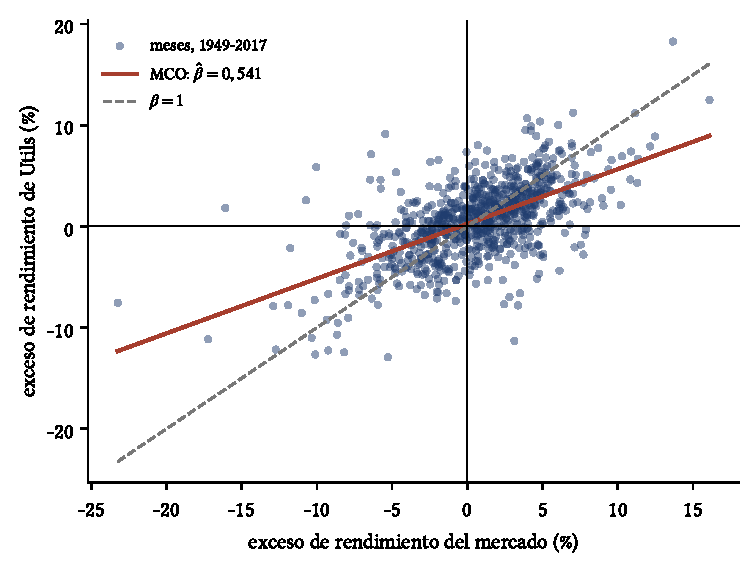
\includegraphics[width=0.66\linewidth]{graficos/cap03_fig_utils.pdf}
\caption{Excesos de rendimiento mensuales de \texttt{Utils} frente al mercado, 1949--2017. La recta MCO
(roja) es mucho más plana que la de $\beta=1$ (gris): el sector amplifica poco los movimientos del mercado.
La gran dispersión vertical alrededor de la recta es el riesgo idiosincrático.}
\label{fig:utils}
\end{figure}

\begin{conclusion}
El sector de servicios públicos tiene una beta de 0,54 y una alfa positiva y significativa de casi 3\,\%
anual. Si el CAPM fuera correcto, las empresas reguladas de este tipo tendrían un costo de capital bajo;
pero el sector rindió más de lo que su beta justifica, lo que anticipa la evidencia de la SML plana del
Ejercicio~\ref{ej:sml}.
\end{conclusion}
\end{ejresuelto}

\begin{ejresuelto}{El modelo de mercado en doce industrias}\label{ej:industrias}
\enunciado Estime el modelo de mercado para las 12 industrias. Reporte la alfa anual, su estadístico $t$,
la beta, el estadístico $t$ de $H_0:\beta=1$ y el $R^2$. ¿Cuántas alfas son significativas al 5\,\%?
¿Hay un patrón entre alfa y beta?

\solucion
\paso{Paso 1. Betas.} Van de 0,54 (\texttt{Utils}) a 1,25 (\texttt{BusEq}: equipos y tecnología). Todas
las betas son distintas de 1 al 5\,\% excepto la de \texttt{Shops} (comercio minorista, $t=-1{,}57$). Las
industrias defensivas (servicios públicos, telecomunicaciones, bienes no durables, energía, salud)
tienen betas menores que 1; las cíclicas (bienes durables, manufactura, tecnología), mayores.

\paso{Paso 2. Alfas.} Cuatro de doce alfas son significativas: \texttt{Utils} ($2{,}96$\,\%, $t=2{,}30$),
\texttt{NoDur} ($2{,}74$\,\%, $t=2{,}87$), \texttt{Hlth} ($3{,}32$\,\%, $t=2{,}49$) y \texttt{Other}
($-1{,}93$\,\%, $t=-2{,}24$). Si el CAPM fuera cierto y las pruebas fueran independientes, esperaríamos
$0{,}05\times12=0{,}6$ rechazos.

\paso{Paso 3. Patrón.} Ordenadas por beta, las alfas tienden a ser positivas en las industrias de beta baja
y negativas en las de beta alta. Las tres alfas positivas significativas corresponden a betas entre 0,54 y
0,87. Este patrón es el mismo que muestra la SML del Ejercicio~\ref{ej:sml}.

\codigoweb{cap03_ej02}
\salidaR{cap03_ej02_R.txt}
\lectura{cap03_ej02}

\RvsPy En R, \texttt{I(d[[i]] - d\$RF)} dentro de la fórmula hace que la resta se interprete como
aritmética y no como sintaxis de fórmulas; \texttt{sapply} recorre las industrias y devuelve una matriz.
En Python, el bucle construye un diccionario de diccionarios que \texttt{pandas} convierte en tabla.

\begin{figure}[ht]
\centering
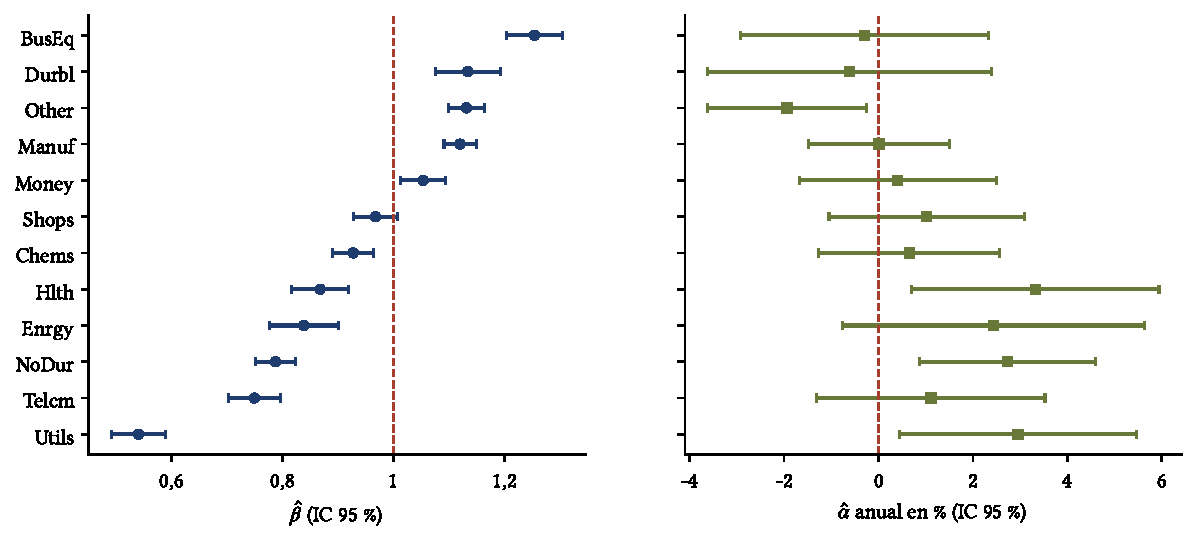
\includegraphics[width=\linewidth]{graficos/cap03_fig_betas.pdf}
\caption{Betas (izquierda) y alfas anuales (derecha) de las 12 industrias con intervalos de confianza al
95\,\%, ordenadas por beta. Las betas se estiman con mucha precisión; las alfas, con mucha menos: la mayoría
de sus intervalos incluyen el cero.}
\label{fig:betas}
\end{figure}

\begin{conclusion}
La beta resume bien la sensibilidad de cada industria al mercado y se estima con precisión. Las alfas, en
cambio, son imprecisas (intervalos de $\pm1{,}5$ a $\pm3{,}2$ puntos anuales) y, cuando son significativas,
siguen un patrón: positivas con beta baja y negativas con beta alta, en contra del CAPM.
\end{conclusion}
\end{ejresuelto}

\begin{ejresuelto}{La recta del mercado de valores es plana}\label{ej:sml}
\enunciado Con las betas del Ejercicio~\ref{ej:industrias} y los excesos de rendimiento promedio de cada
industria (anualizados), estime la regresión de corte transversal $\bar Z_i=\gamma_0+\gamma_1\hat\beta_i+u_i$
y compárela con la predicción del CAPM ($\gamma_0=0$, $\gamma_1=$ prima de mercado).

\solucion
\paso{Paso 1. Prima de mercado.} El exceso de rendimiento promedio del mercado es $7{,}74$\,\% anual; esa
es la pendiente que predice el CAPM.

\paso{Paso 2. Estimación.} $\hat\gamma_0=7{,}05$ ($t=4{,}89$) y $\hat\gamma_1=1{,}34$ ($t=0{,}90$), con
$R^2=0{,}075$. Comparada con la teórica, la pendiente estimada es
\begin{align*}
  \frac{\hat\gamma_1}{\bar Z_m} &= \frac{1{,}344}{7{,}744}\\
                                &= 0{,}17,
\end{align*}
menos de una quinta parte, y no es significativa; el intercepto, que debería ser cero, es grande y
significativo.

\paso{Paso 3. Interpretación.} En este período, una industria con beta 0,5 ganó en promedio casi lo
mismo que una con beta 1,25: la beta casi no explica las diferencias de rendimiento entre industrias. Es el
resultado clásico de Black, Jensen y Scholes (1972) y Fama y French (1992): la SML empírica es más plana
que la teórica.

\paso{Paso 4. Advertencias.} Con solo 12 observaciones la prueba de corte transversal tiene poca potencia.
Además, las betas son estimaciones con error: el error de medición en el regresor sesga $\hat\gamma_1$ hacia
cero (sesgo de atenuación). Con $\operatorname{ee}(\hat\beta)$ entre 0,015 y 0,032 y betas que varían de
0,54 a 1,25, el factor de atenuación estimado es de 0,99 (Ejercicio propuesto~3.4): el sesgo es mínimo y no
explica una pendiente tan plana.

\codigoweb{cap03_ej03}
\salidaR{cap03_ej03_R.txt}
\lectura{cap03_ej03}

\RvsPy En los dos lenguajes la regresión de corte transversal es una regresión ordinaria con 12
observaciones. En Python, \texttt{beta.rename("beta")} sirve solo para que el coeficiente aparezca con un
nombre legible en la tabla de resultados.

\begin{figure}[ht]
\centering
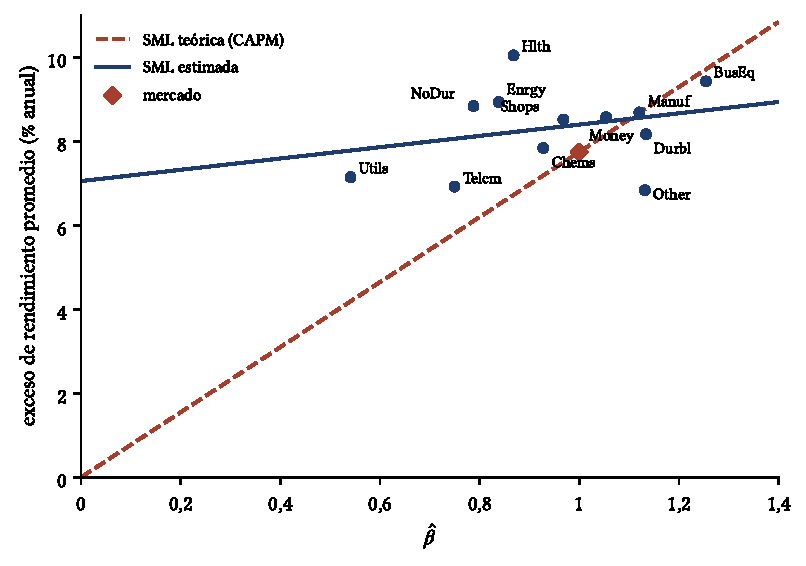
\includegraphics[width=0.74\linewidth]{graficos/cap03_fig_sml.pdf}
\caption{Recta del mercado de valores, 1949--2017. La línea discontinua es la predicción del CAPM: pasa
por el origen y por el mercado. La línea continua es la estimada con las 12 industrias: mucho más plana.
Las industrias de beta baja quedan por encima de la teórica (alfa positiva) y las de beta alta, por debajo.}
\label{fig:sml}
\end{figure}

\begin{conclusion}
Los datos no apoyan la predicción central del CAPM: los activos de beta alta no ganaron más que los de beta
baja en la proporción que el modelo predice. Esto no significa que la beta sea inútil (mide bien el riesgo
de mercado, Ejercicio~\ref{ej:industrias}), sino que no basta para explicar los rendimientos esperados. Los
modelos multifactoriales del Capítulo~14 nacen de esta evidencia.
\end{conclusion}
\end{ejresuelto}

\begin{ejresuelto}{¿Son estables las betas?}\label{ej:movil}
\enunciado Estime betas móviles con ventanas de 60 meses para \texttt{Utils}, \texttt{Enrgy} y
\texttt{BusEq}. Reporte su mínimo, máximo, último valor y desviación estándar, y discuta qué implica para
el uso de la beta en la práctica.

\solucion
\paso{Paso 1. Resultados.} La beta de \texttt{Utils} varió entre $-0{,}01$ (ventana que termina en marzo de
2001) y $0{,}81$ (agosto de 1974). La de \texttt{Enrgy}, entre $0{,}41$ (febrero de 1993) y $1{,}31$
(julio de 1982). La de \texttt{BusEq}, entre $1{,}00$ (noviembre de 2013) y $2{,}02$ (octubre de 2004).

\paso{Paso 2. Lectura económica.} La beta de tecnología se duplicó durante la burbuja de las empresas
puntocom: en la ventana 2000--2004 el mercado subía y bajaba al ritmo de las tecnológicas. En esos mismos
años la beta de servicios públicos llegó a cero: el sector se desacopló de un mercado dominado por la
tecnología. La beta de energía subió en la crisis petrolera de comienzos de los ochenta y en la caída de
precios de 2014--2016.

\paso{Paso 3. Magnitud.} La desviación estándar de las betas móviles (0,17 a 0,23) es de siete a nueve veces el
error estándar de las betas de muestra completa del Ejercicio~\ref{ej:industrias}: la incertidumbre que importa
en la práctica no es el error de estimación, sino el cambio de la beta en el tiempo.

\codigoweb{cap03_ej04}
\salidaR{cap03_ej04_R.txt}
\lectura{cap03_ej04}

\RvsPy En R se recorre cada ventana con \texttt{sapply}. En Python, \texttt{rolling(60).cov()} y
\texttt{rolling(60).var()} de \texttt{pandas} calculan todas las ventanas de una vez, de forma mucho más
rápida. Ambos usan el divisor $n-1$ en covarianza y varianza, que se cancela en el cociente.

\begin{figure}[ht]
\centering
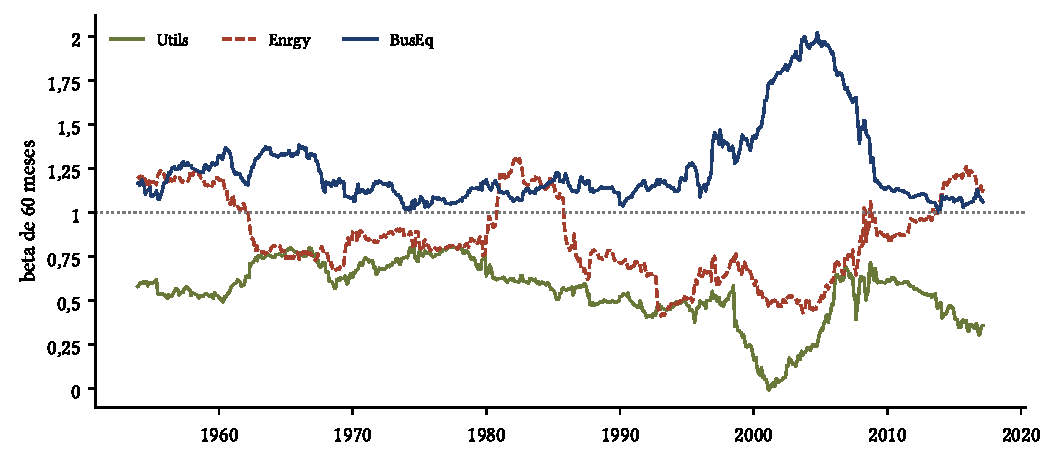
\includegraphics[width=0.92\linewidth]{graficos/cap03_fig_movil.pdf}
\caption{Betas móviles de 60 meses (cada punto usa los cinco años previos). Las betas cambian mucho: la de
tecnología (\texttt{BusEq}) llega a 2 en la burbuja puntocom, y la de servicios públicos (\texttt{Utils})
cae a cero en los mismos años.}
\label{fig:movil}
\end{figure}

\begin{conclusion}
Las betas no son constantes. Una beta estimada con cinco años de datos puede ser muy distinta de la que
regirá en los próximos cinco. En aplicaciones como el costo de capital conviene reportar la beta junto con
su evolución reciente y no como un número fijo.
\end{conclusion}
\end{ejresuelto}

\begin{ejresuelto}{El portafolio tangente y la crítica de Roll}\label{ej:roll}
\enunciado Con las 12 industrias: (a) calcule el portafolio tangente muestral (Corolario~\ref{cor:tangente})
y compare su razón de Sharpe con la del mercado; (b) verifique numéricamente el Teorema~\ref{teo:betarend}
con ese portafolio; (c) repita con el mercado y explique la diferencia.

\solucion
\paso{Paso 1. Pesos.} El portafolio tangente pone $64{,}9$\,\% en bienes no durables y vende en corto
$87{,}1$\,\% en ``otras'' industrias y $26{,}8$\,\% en químicos, entre otras posiciones. Su razón de
Sharpe anual es $0{,}809$, frente a $0{,}527$ del mercado.

\paso{Paso 2. Verificación del teorema.} Con las betas respecto del tangente, la máxima diferencia
$|\mu_i-\beta_{iq}\mu_q|$ es del orden de $10^{-18}$: cero con precisión de máquina. La SML se cumple
\emph{exactamente} en la muestra, como garantiza el Teorema~\ref{teo:betarend}.

\paso{Paso 3. Con el mercado.} Respecto del mercado, la alfa máxima es de $3{,}32$\,\% anual (salud). El
mercado no es el portafolio eficiente de estas 12 industrias en la muestra, y por eso aparecen alfas.

\paso{Paso 4. La lección de Roll.} La SML con el portafolio tangente no ``confirma'' nada: es una identidad
matemática. Y el portafolio tangente muestral no es un portafolio que alguien hubiera podido elegir en 1949,
porque usa medias y covarianzas que solo se conocen al final; sus posiciones cortas extremas son señal de que
optimiza el ruido de la muestra. Contrastar el CAPM es contrastar si el índice de mercado es eficiente, y la
respuesta depende de qué activos se incluyan.

\codigoweb{cap03_ej05}
\salidaR{cap03_ej05_R.txt}
\lectura{cap03_ej05}

\RvsPy Para obtener $\bm\Sigma^{-1}\bm\mu$ no conviene invertir la matriz: \texttt{solve(S, mu)} en R y
\texttt{np.linalg.solve(S, mu)} en Python resuelven el sistema lineal directamente, lo que es más rápido y
numéricamente más estable. La diferencia de $3{,}5\times10^{-18}$ (R) frente a $9{,}5\times10^{-18}$ (Python) en
el Paso~2 es solo error de redondeo de punto flotante.

\begin{figure}[ht]
\centering
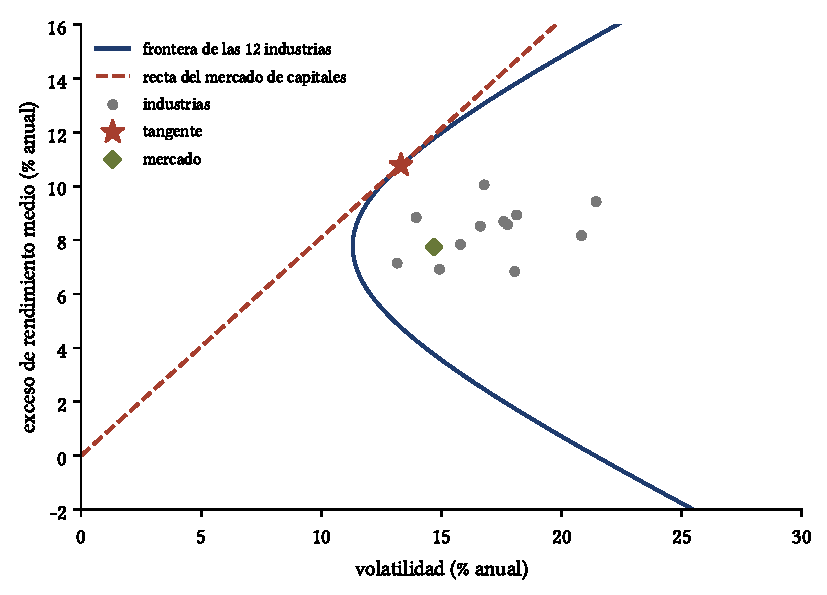
\includegraphics[width=0.74\linewidth]{graficos/cap03_fig_frontera.pdf}
\caption{Frontera de mínima varianza de las 12 industrias, 1949--2017, con la recta del mercado de capitales
que toca la frontera en el portafolio tangente (estrella). El mercado (rombo) queda dentro de la frontera:
no es eficiente con respecto a estas 12 industrias en la muestra.}
\label{fig:frontera}
\end{figure}

\begin{conclusion}
Respecto de un portafolio eficiente, la relación beta-rendimiento siempre se cumple; el CAPM tiene contenido
solo porque afirma que el mercado es ese portafolio. Con estos datos, el índice de mercado no es eficiente
respecto de las 12 industrias, lo que es otra forma de ver las alfas del Ejercicio~\ref{ej:industrias}.
\end{conclusion}
\end{ejresuelto}

% ---------------------------------------------------------------------
\section{Ejercicios propuestos}
% ---------------------------------------------------------------------

\begin{enumerate}[label=\textbf{\thechapter.\arabic*},leftmargin=*,itemsep=6pt]
  \item Demuestre que en la regresión MCO con constante se cumplen $\sum_t\hat\varepsilon_t=0$ y
  $\sum_tx_t\hat\varepsilon_t=0$, y que la recta pasa por el punto $(\bar x,\bar y)$. Use estas propiedades
  para demostrar que $\Var(y)=\hat\beta^2\Var(x)+\Var(\hat\varepsilon)$ en la muestra, como verificó el
  Ejercicio~\ref{ej:utils}.

  \item Demuestre que la beta de un portafolio es el promedio ponderado de las betas de los activos que lo
  forman, con los pesos del portafolio. ¿Qué beta tiene un portafolio con 50\,\% en \texttt{Utils} y
  50\,\% en \texttt{BusEq}? \textit{Respuesta: $0{,}5\times0{,}541+0{,}5\times1{,}254=0{,}898$.}

  \item Suponga que se regresa $Z_{it}$ sobre $Z_{mt}$ sin constante. Demuestre que la pendiente estimada es
  $\sum_tx_ty_t/\sum_tx_t^2$ y que difiere de $\hat\beta$ salvo que $\hat\alpha=0$ o $\bar x=0$.

  \item (Sesgo de atenuación.) Si $\hat\beta_i=\beta_i+v_i$ con $v_i$ independiente de $\beta_i$ y de varianza
  $\sigma^2_v$, demuestre que la pendiente de la regresión de $\bar Z_i$ sobre $\hat\beta_i$ converge a
  $\gamma_1\,\Var(\beta)/[\Var(\beta)+\sigma^2_v]$. Con los datos del Ejercicio~\ref{ej:industrias},
  estime el factor de atenuación. \textit{Pista: aproxime $\Var(\beta)$ por la varianza muestral de las
  betas menos el promedio de los $\operatorname{ee}^2$.}

  \item Demuestre la segunda parte del Corolario~\ref{cor:tangente}: la razón de Sharpe del portafolio
  tangente es $\sqrt{\bm\mu'\bm\Sigma^{-1}\bm\mu}$ y ningún otro portafolio tiene una razón mayor.
  \textit{Pista: use la desigualdad de Cauchy-Schwarz con el producto interno $\langle a,b\rangle=a'\bm\Sigma b$.}

  \item \emph{(Con datos.)} Divida la muestra en 1949--1982 y 1983--2017 y repita el
  Ejercicio~\ref{ej:sml} en cada mitad. ¿Es la SML plana en ambos períodos?

  \item \emph{(Con datos del Capítulo~\ref{cap:rendimientos}.)} Estime la beta de Credicorp, Southern Copper
  y Buenaventura respecto del índice S\&P/BVL Perú General, con rendimientos mensuales en soles y la tasa
  interbancaria del BCRP como tasa libre de riesgo. ¿Cuál es la acción más defensiva? ¿Cambian las betas
  si se usa el S\&P 500 como mercado?

  \item \emph{(Investigación.)} En la regulación tarifaria peruana, el costo de capital de las empresas de
  servicios públicos suele estimarse con un CAPM adaptado a mercados emergentes. Busque cómo lo calcula
  un organismo regulador peruano (por ejemplo, OSINERGMIN o SUNASS) y discuta qué beta usa y por qué.
\end{enumerate}

% ---------------------------------------------------------------------
\section{Resumen de fórmulas}
% ---------------------------------------------------------------------

\begin{table}[H]
\centering\small
\begin{tabular}{@{}ll@{}}
\toprule
Concepto & Fórmula \\
\midrule
Modelo de mercado & $Z_{it}=\alpha_i+\beta_iZ_{mt}+\varepsilon_{it}$ \\
Beta & $\beta_i=\Cov(Z_i,Z_m)/\Var(Z_m)$;\quad $\hat\beta=S_{xy}/S_{xx}$ \\
Alfa & $\hat\alpha=\bar y-\hat\beta\bar x$ \\
Riesgo total & $\Var(Z_i)=\beta_i^2\Var(Z_m)+\Var(\varepsilon_i)$;\quad $R^2=\rho^2(Z_i,Z_m)$ \\
Errores estándar & $\operatorname{ee}(\hat\beta)=\sqrt{s^2/S_{xx}}$;\quad $\operatorname{ee}(\hat\alpha)=\sqrt{s^2(1/T+\bar x^2/S_{xx})}$ \\
Relación beta-rendimiento & $\mu_i=\beta_{iq}\mu_q$ si $q$ es eficiente \\
Portafolio tangente & $\bm w_q=\bm\Sigma^{-1}\bm\mu/(\bm1'\bm\Sigma^{-1}\bm\mu)$;\quad $SR_q=\sqrt{\bm\mu'\bm\Sigma^{-1}\bm\mu}$ \\
SML de corte transversal & $\bar Z_i=\gamma_0+\gamma_1\hat\beta_i+u_i$;\quad CAPM: $\gamma_0=0$, $\gamma_1=\bar Z_m$ \\
\bottomrule
\end{tabular}
\caption{Fórmulas principales del Capítulo 3.}
\end{table}

\section*{Referencias}
\begin{itemize}[leftmargin=*]
  \item Black, F., Jensen, M. C. y Scholes, M. (1972). The capital asset pricing model: some empirical
        tests. En M. C. Jensen (ed.), \emph{Studies in the Theory of Capital Markets}. Praeger.
  \item Fama, E. F. y French, K. R. (1992). The cross-section of expected stock returns. \emph{The Journal
        of Finance}, 47(2), 427--465.
  \item French, K. R. \emph{Data Library}. Tuck School of Business, Dartmouth College.
        \url{https://mba.tuck.dartmouth.edu/pages/faculty/ken.french/data_library.html}.
  \item Gibbons, M. R., Ross, S. A. y Shanken, J. (1989). A test of the efficiency of a given portfolio.
        \emph{Econometrica}, 57(5), 1121--1152.
  \item Lintner, J. (1965). The valuation of risk assets and the selection of risky investments in stock
        portfolios and capital budgets. \emph{The Review of Economics and Statistics}, 47(1), 13--37.
  \item Roll, R. (1977). A critique of the asset pricing theory's tests. Part I: On past and potential
        testability of the theory. \emph{Journal of Financial Economics}, 4(2), 129--176.
  \item Sharpe, W. F. (1964). Capital asset prices: a theory of market equilibrium under conditions of
        risk. \emph{The Journal of Finance}, 19(3), 425--442.
  \item Wooldridge, J. M. (2020). \emph{Introductory Econometrics: A Modern Approach} (7.ª ed.). Cengage.
\end{itemize}
